\chapter{Introduction}
\label{ch:introduction}

\section{The Earth’s radiation budget}
The Earth's climate is driven by the energy flow into and out of the system. The incoming solar radiation (yellow fluxes in \figref{fig:earth_energy_budget}) reaches the Earth at the top of the atmosphere (TOA), then goes through the atmosphere and arrives at the Earth surface. During this process, approximately two thirds of this shortwave (SW) radiation is absorbed by the Earth surface and atmosphere, and roughly one third of this energy is reflected back to space. The the surface and atmosphere are heated by this incoming solar radiation, and they also re-emit the longwave (LW) radiation (purple fluxes in \figref{fig:earth_energy_budget}) to keep a relatively stable temperature. Globally, the annual mean incoming solar radiation flux is about 340 Wm$^{-2}$, the reflected solar radiation flux is around 100 Wm$^{-2}$ and the outgoing longwave radiation (OLR) is close to 240 Wm$^{-2}$ at the TOA for period 2000--2010 \citep{Stephens2012update}. These three components balance with each other, with a small positive imbalance (about 0.6 Wm$^{-2}$) at the TOA. A more recent estimate from \cite{Wild2015} (see their Fig. 1) indicates that the gloabl mean OLR is about 239 Wm$^{-2}$, and the TOA energy imbalance is about 1 Wm$^{-2}$.
%But due to the accuracy of the observation itself, it is hard to track the causes of these imbalance.

\begin{figure}[ht]
	\centering
	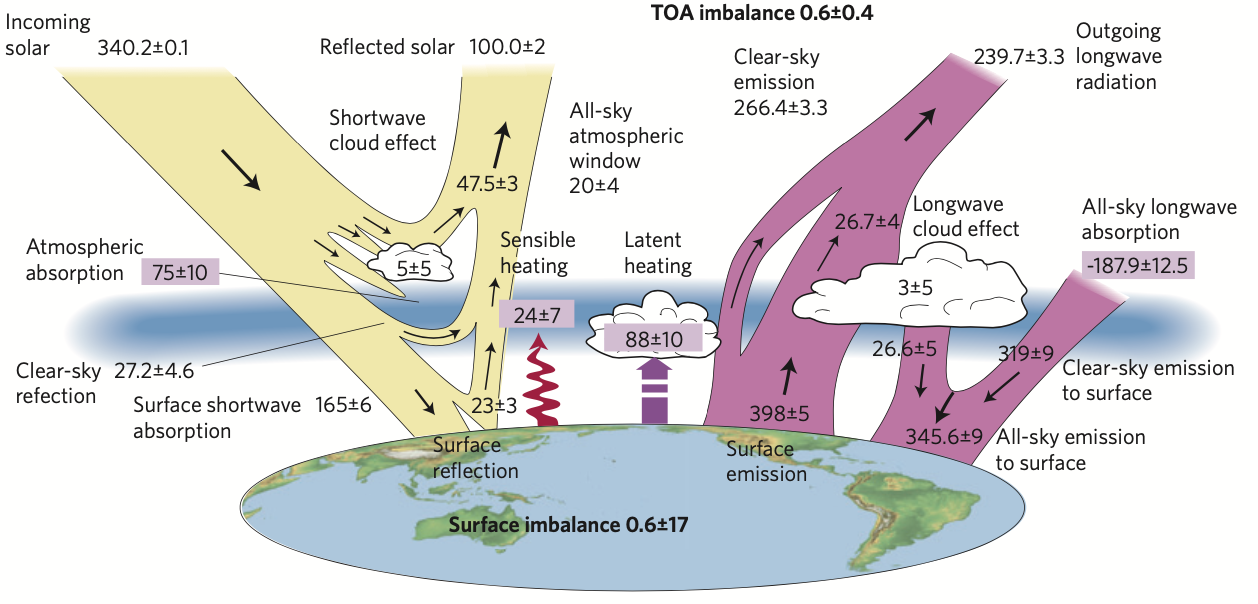
\includegraphics[width=1\linewidth]{{figs/literature_review/earth_enery_budget_Stephens2012}.png}
	\caption[The global annual mean energy budget of Earth for the approximate period 2000–2010 from \cite{Stephens2012update}]{The global annual mean energy budget of Earth for the approximate period 2000–2010. All fluxes are in Wm$^{-2}$. Solar fluxes are in yellow and infrared fluxes in purple. The four flux quantities in purple-shaded boxes represent the principal components of the atmospheric energy balance. Adapted from \cite{Stephens2012update}.}
	\label{fig:earth_energy_budget}
\end{figure}

As shown in \figref{fig:earth_energy_budget}, the energy budget at the Earth's surface is more complicated than at the TOA. When the incoming solar radiation reaches the surface, the majority (about 165 Wm$^{-2}$) of this solar radiation is absorbed by the surface and only a small portion (about 23 Wm$^{-2}$) is reflected back to space. Of course, these are global mean results and it would be different over certain areas such as Arctic where the surface albedo is large. The global annual mean LW radiation emitted from the surface is about 398 Wm$^{-2}$. Much of this is absorbed by the atmosphere (such as the greenhouse gases, aerosols and clouds), and only a small part (about 20 Wm$^{-2}$) can pass through the atmospheric window region (a portion of the infrared spectrum where there is almost no atmospheric absorption) reaching the TOA directly. The atmosphere can re-emit the absorbed LW radiation both upward and downward, and downward part (about 346 Wm$^{-2}$) can reheat the surface. In addition, due to the temperature and moisture difference between the surface and atmosphere, the surface is also cooled by the latent heat flux (about 88 Wm$^{-2}$) and sensible heat flux (about 24 Wm$^{-2}$) through the turbulent movement of atmosphere. In total, the surface energy budget is balanced by the downward/upward SW and LW radiation, the sensible and latent heat fluxes, but it has much larger uncertainty than at the TOA.


\section{Clouds and cloud radiative effect}

Clouds usually cover more than half areas of the Earth at any given time \citep{Houze2014,Ramanathan1989}, which is supported by recent International Satellite Cloud Climatology Project (ISCCP)\index{ISCCP} H-series products \citep{Young2018}, as shown in \tabref{tab:statistics_cld_amt}. Although they vary among different regions, the cloud amounts are usually larger over ocean regions than over lands, as the ocean provides a abundance of water vapor.

\begin{table}[htp]
\centering
%\scriptsize
\caption{Statistics of the annually averaged total cloud amount (\%) for various regions, which are from the ISCCP H-series data sets \citep{Young2018} from 1984 to 2014.}
\vspace{0.5em}
\begin{tabular}{cccc}
	\toprule
	Region & Ocean & Land &  Total\\
	\midrule
	Global & 71.7 & 54.8 & 66.1 \\
	15$^\circ$S--15$^\circ$N&  62.4&  63.5& 62.6 \\
	15$^\circ$N--35$^\circ$N&  60.1&  46.6& 55.2\\
	15$^\circ$S--35$^\circ$S&  65.0&  48.3& 61.4\\
	35$^\circ$N--60$^\circ$N&  80.9&  64.6& 72.5 \\
	35$^\circ$S--60$^\circ$S&  84.0&  65.0& 83.5 \\
	60$^\circ$N--90$^\circ$N&  68.9&  62.0& 66.5\\
	60$^\circ$S--90$^\circ$S&  80.1&  44.3& 60.1 \\
	\bottomrule
\end{tabular}
\label{tab:statistics_cld_amt}
\end{table}

\begin{figure}[ht]
	\centering
	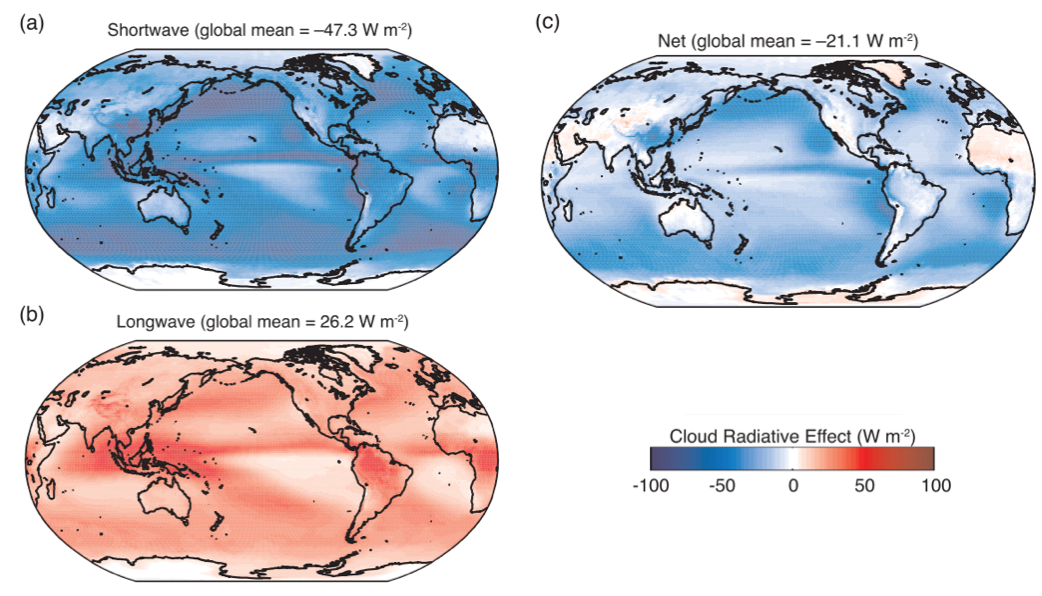
\includegraphics[width=1\linewidth]{{figs/literature_review/spatial_pattern_of_CRE_from_IPCC_ch7}.png}
	\caption{Distribution of annual-mean top of the atmosphere (a) shortwave, (b) longwave, (c) net cloud radiative effects averaged over the period 2001–2011 from the Clouds and the Earth’s Radiant Energy System (CERES) Energy Balanced and Filled (EBAF) Ed2.6r data set. Adapted from Fig. 7.7 of The Fifth Assessment Report (AR5) of the Intergovernmental Panel on Climate Change (IPCC) \citep{stocker2013climate}.}
	\label{fig:CRE_from_IPCC}
\end{figure}

\section{Cloud feedback}

\section{Cloud scheme}

\section{Research questions and thesis outline}
\label{sec:thesis_layout}
